\documentclass[]{article}
\usepackage[utf8]{inputenc}
\usepackage{polski}
\usepackage{listings}
\usepackage[usenames,dvipsnames]{xcolor}
\usepackage{geometry}
\usepackage{subcaption}
\usepackage{graphicx}
\usepackage{amsmath}
\usepackage{amssymb}
\usepackage{enumerate}
\usepackage[font=small]{caption}
\usepackage[ruled,noend]{algorithm2e}
\SetAlgorithmName{Algorytm}{algorytm}{Algorytmy}
\DeclareGraphicsExtensions{.png}
\graphicspath{ {./} }
\geometry{
	a4paper,
	left=25mm,
	right = 25mm,
	top=20mm,
	bottom=20mm
}
%%\hyphenchar\font=-1

\title{
	Sprawozdanie \\
	\large 
	Obliczenia naukowe - lista 4}
\author{Kamil Król}
\date{244949}


\begin{document}
	
	\maketitle
	
	\section*{Zadanie 1}
	Celem tego zadania było napisanie funkcji w języku Julia, która oblicza ilorazy różnicowe. Dodatkowym wymaganiem było nieużywanie tablicy dwuwymiarowej.\\
	\textbf{Dane:}
	\begin{enumerate}[]
		\item \texttt{x} -- wektor długości $n+1$ zawierający węzły $x_0, \ldots, x_n$,
		\item \texttt{f} -- wektor długości $n+1$ zawierający wartości interpolowanej funkcji w poprzednio podanych\\ węzłach tj. $f(x_0), \ldots, f(x_n)$.
	\end{enumerate}
	\textbf{Oczekiwany wynik:}
	\begin{enumerate}[]
		\item fx –- wektor długości n + 1 zawierający obliczone ilorazy różnicowe
	\end{enumerate}
	\textbf{Opis:}\\
	Najpierw przyjrzyjmy się temu w jaki sposób można obliczyć ilorazy różnicowe.
	Poniżej znajduje się wzór rekurencyjny pozwalający na obliczenie ilorazu różnicowego k-tego rzędu.
	\begin{enumerate}[]
		\item dla $k = 0$  $$f[x_i] = f(x_i),$$
		\item dla $k = 1$  $$f[x_i,x_j] = \frac{f(x_j) - f(x_i)}{x_j - x_i},$$  
		\item dla $k > 1$  $$f[x_i,x_{i+1}, \ldots, x_{i+k}] = \frac{f[x_{i+1},x_{i+2}, \ldots, x_{i+k}] - f[x_{i}, x_{i+1}, \ldots, x_{i+k-1}]}{x_k - x_i}.$$
	\end{enumerate}
	Ważnym faktem jest to, że wartość ilorazu różnicowego nie zależy od kolejności węzłów ($x_i$). Kolejny użyteczny fakt to to, że 
	znajomość węzłów $x_i$ i wartości funkcji $f(x_i)$ (a więc też ilorazów różnicowych zerowego rzędu tj. $f[x_i] = f(x_i)$) pozwala, przy użyciu powyższego wzoru rekurencyjnego, na stworzenie tzw. tablicy ilorazów różnicowych dla wyższych rzędów. Przyjmując, że $d_{ik} = f[x_i,x_{i+1}, \ldots, x_{i+k}]$ można wyrazić ją w następujący sposób:
\begin{table}[!htbp]
	\centering
	\begin{tabular}{cccccc}
		$d_{0,0}$ & $d_{0,1}$ & $d_{0,2}$ & \ldots & $d_{0,k-1}$ & $d_{0,k}$ \\
		$d_{1,0}$ & $d_{1,1}$ & $d_{1,2}$ &\ldots & $d_{1,k-1}$ & \\
		\ldots & \ldots & \ldots & \ldots && \\
		$d_{k-1,0}$ & $d_{k-1,1}$ & $d_{k-1,2}$ &&& \\
		$d_{k-1,0}$ & $d_{k-1,1}$ &&&& \\
		$d_{k,0}$ &&&&& \\
	\end{tabular}
\end{table}

	\noindent Pierwsza intuicja co do zaprogramowania funkcji obliczającej ilorazy różnicowe to użycie macierzy -- tablicy dwuwymiarowej. Zastanówmy się najpierw czy można to zrobić bardziej efektywnie i jakich danych z powyższej tablicy ilorazów różnicowych potrzebujemy. Interesujące dla nas są tylko dane w pierwszym wierszu tej tablicy. Jeśli dodatkowo zauważymy, że każda kolumna zależy tylko i wyłącznie od poprzedniej kolumny możemy zaproponować rozwiązanie używające tablicy jednowymiarowej. W pierwszym kroku powinniśmy zapisać wartości pierwszej kolumny do jednowymiarowej tablicy. Te dane już mamy, ponieważ są to wartości funkcji w danych węzłach. (Przypomnijmy, że $f[x_i] = f(x_i)$). Następnie w każdym kolejnym kroku powinniśmy wpisywać odpowiednie
	wartości z kolejnych kolumn na ostatnie miejsca w tablicy. W rezultacie w naszej tablicy otrzymamy tylko wartości ilorazów z pierwszego wiersza.\\
	\clearpage
	\noindent\textbf{Pseudokod algorytmu}\\
	\begin{algorithm}[h]
		\DontPrintSemicolon
		\SetKwProg{Fn}{function}{}{}
		\SetKw{KwDownTo}{downto}
		
		\SetKwFunction{ir}{ilorazyRoznicowe}
		\SetKwFunction{len}{length}
		
		\Fn{\ir{$x$,$f$}}{
			\For{$i \gets 1$ \KwTo \len{$f$}} {
				$fx[i] \gets f[i]$\;
			}
			\For{$i \gets 1$ \KwTo \len{$f$}} {
				
				\For{$j \gets$\len{$f$} \KwDownTo $i$} {
					$fx[j] \gets \dfrac{fx[j]-fx[j-1]}{x[j] - x[j-i]}$\;
					
				}
			}
			
			\KwRet $fx$\;
		}
		\caption{Obliczanie ilorazów różnicowych}
	\end{algorithm}
	
	\section*{Zadanie 2}
	
	Celem tego zadania było napisanie funkcji obliczającej wartość wielomianu interpolacyjnego stopnia $n$ w postaci Newtona $N_{n}(x)$ w punkcie $x = t$ za pomocą uogólnionego algorytmu Hornera, która działa w czasie liniowym ($O(n)$). \\
	\textbf{Dane:}
	\begin{enumerate}[]
		\item \texttt{x} -- wektor długości $n+1$ zawierający węzły $x_0, \ldots, x_n$,
		\item \texttt{fx} -- wektor długości $n+1$ zawierający ilorazy różnicowe,
		\item \texttt{t} -- punkt, w którym należy obliczyć wartość wielomianu.
	\end{enumerate}
	\textbf{Oczekiwany wynik:}
	\begin{enumerate}[]
		\item \texttt{nt} -- wartość wielomianu w punkcie $t$
	\end{enumerate}
	\textbf{Opis:}\\
	\noindent Wzór na wielomian interpolacyjny Newtona $N_n$ pokazuje w jaki sposób zależy on od funkcji $f$. Wzór ten można przedstawić używając ilorazów różnicowych:
	$$N_n(x) = \sum_{i=0}^n f[x_0,x_{1}, \ldots, x_{i}] \prod_{j=0}^{i-1}(x-x_j).$$
	Z numerycznego punktu widzenia takie przedstawienie wielomianu interpolacyjnego jest bardzo atrakcyjne. Zauważmy, że w sytuacji kiedy chcielibyśmy dodać nowe węzły $(x_i, y_i)$ możemy to zrobić korzystając ze wcześniej policzonych $d_k = f[x_0,x_1, \ldots, x_k]$. Kluczowa jest tu własność ilorazów różnicowych mówiąca, że wartość ilorazu nie zależy od kolejności węzłów. Kolejną zaletą takiego zapisu jest to, że wartość tego wielomianu możemy łatwo obliczyć korzystając z uogólnionego algorytmu Hornera. Sposób w jaki można to zrobić przedstawiono poniżej.
	\begin{align*}
	&w_n(x) := f[x_0, x_1, \ldots, x_n]& \nonumber \\
	&w_k(x) := w_{k+1}(x-x_k)+ f[x_0, x_1, \ldots, x_k]	\quad(k=n-1, n-2, \ldots, 0)& \nonumber \\
	&N_n(x) = w_0(x) \nonumber \\
	\end{align*}
	\clearpage
	\noindent\textbf{Pseudokod algorytmu}\\
	\begin{algorithm}[h]
		\DontPrintSemicolon
		\SetKw{KwDownTo}{downto}
		\SetKwProg{Fun}{function}{}{}
		\SetKwFunction{LEN}{length}
		\SetKwFunction{F}{warNewton}
		
		\Fun{\F{$x$, $fx$, $t$}} {
			$n \gets \LEN{fx}$\;
			$nt \gets fx[n]$\;
			\For{$i \gets n-1$ \KwDownTo $1$} {
				$nt \gets fx[i] + (t - x[i]) \times nt$\; 		
			}
			\KwRet $nt$\;
		}
		\caption{Obliczanie wartości wielomianu interpolacyjnego w punkcie $t$.}
	\end{algorithm}			
	
	

	\section*{Zadanie 3} 
	
	Celem tego zadania było napisanie funkcji obliczającej współczynniki $a_0,\ldots,a_n$ postaci naturalnej wielomianu interpolacyjnego dla zadanych współczynników $d_0 = f[x_0], d_1 = f[x_0,x_1], \ldots d_n = f[x_0, \ldots, x_n]$ tego wielomianu w postaci Newtona oraz węzłów $x_0, \ldots, x_n$. Ponadto funkcja miała działać w czasie $O(n^2)$.\\
	\textbf{Dane:}
	\begin{enumerate}[]
		\item \texttt{x} -- wektor długości $n+1$ zawierający węzły $x_0, \ldots, x_n$,
		\item \texttt{fx} -- wektor długości $n+1$ zawierający ilorazy różnicowe.
	\end{enumerate}
	\textbf{Oczekiwany wynik:}
	\begin{enumerate}[]
		\item \texttt{a} -- wektor długości $n+1$ zawierający obliczone współczynniki postaci naturalnej.
	\end{enumerate}
	\textbf{Opis:}\\
	Przypomnijmy, że wartości $d_0, d_1, \ldots, d_n$ są współczynnikami wielomianu interpolacyjnego w postaci Newtona. Punktem wyjściowym to wyprowadzenia algorytmu będzie uogólniony algorytm Hornera. Najpierw jednak zapiszmy wielomian interpolacyjny w postaci Newtona: 
	$$ p(x) = \underbrace{d_0 + (x-x_0)(\underbrace{d_1 + (x-x_1)
	(d_2 + \ldots + (x-x_{n-2})(\overbrace{d_{n-1}+(x-x_{n-1})\underbrace{d_n}_{W_n}}^{W_{n-1}}))}_{W_1}}_{W_0}\ldots)$$

	\noindent Idea jest bardzo podobna do wyprowadzania uogólnionego algorytmu Hornera w poprzednim zadaniu. Teraz przyjrzyjmy się zaznaczonym wielomianom $W_k$. Zauważmy też, że ich stopnie rosną (patrząc od góry do dołu).
	\begin{align*}
	W_n(x) & = d_n\nonumber \\
	W_{n-1}(x) &= d_{n-1} + (x-x_{n-1})W_n \nonumber \\
	\ldots & = \ldots \\
	W_k(x) &= d_{k} + (x - x_{k})W_{k+1} \text{ dla } 0\le k<n \nonumber \\
	\ldots & = \ldots \\
	W_0(x) &= p_0(x) \nonumber \\
	\end{align*}
	\clearpage
	Dodatkowo mamy też, że $deg(W_k) = deg(W_{k+1}) + 1$. Obie te obserwacje są kluczowe dla wyprowadzenia algorytmu. Przypomnijmy, że wartości $d_0, d_1, \ldots, d_n$ oraz $x_0, \ldots, x_n$ są danymi, a więc są znane.
	Zastanówmy się jak obliczyć współczynniki wielomianu $W_{n-1}$ w postaci naturalnej. Mamy $deg(W_{n-1}) = deg(W_n) + 1 = 0 + 1 = 1$, a zatem $W_{n-1}$ możemy ogólnie zapisać jako $W_{n-1}(x) = a_{0}x^0 + a_{1}x^1$. Z drugiej strony patrząc na tabelę wyżej możemy go zapisać jako $$W_{n-1}(x) = d_{n-1} + (x - x_{n-1})W_n = d_{n-1} + (x - x_{n-1})d_n = d_{n-1} + xd_n - x_{n-1}d_n = 
	(d_{n-1} - d_nx_{n-1})x^0 + (d_{n})x^1 $$
	Otrzymaliśmy współczynniki naturalne wielomianu $W_{n-1}$. Konkretniej mamy, że $a_0=d_{n-1} - d_nx_{n-1}$ i $a_1=d_{n}$. Zróbmy to samo dla $W_{n-2}$. $$W_{n-2}(x)=d_{n-2}+(x-x_{n-2})W_{n-1} =d_{n-2}+(x-x_{n-2})(a_{0}x^0 + a_{1}x^1) = $$
	$$(d_{n-2} - x_{n-2}a_0)x^0 + (a_0-a_1x_{n-2})x^1 + a_1x^2$$
	Obliczyliśmy współczynniki $W_{n-2}$ w postaci naturalnej. Jeśli ten wielomian zapiszemy jako $W_{n-2} = b_0x^0+b_1x^1+b_2x^2$ to współczynniki będą następujące: $b_0 = d_{n-2} - x_{n-2}a_0$, $b_1=a_0-a_1x_{n-2}$, $b_2=a_1$.
	Widzimy zatem, że współczynniki przy najwyższej potędze wielomianów $W_{n-1}$ i $W_{n-2}$ są sobie równe. Ogólnie mamy, że współczynniki przy najwyższej potędze dla wielomianów $W_{k}$ i $W_{k-1}$ są sobie równe. Inna kluczowa obserwacja to fakt, że licząc współczynniki naturalne wielomianu $W_{n-2}$ korzystaliśmy tylko z danych i ze współczynników naturalnych wielomianu $W_{n-1}$. Podobnie obliczając współczynniki wielomianu $W_{n-1}$ korzystaliśmy tylko z danych i współczynników wielomianu $W_{n}$. Widzimy zatem, że współczynniki naturalne wielomianu $W_k$ jesteśmy w stanie obliczyć znając współczynniki wielomianu $W_{k+1}$. Oznacza to, że możemy to zrobić używając jednej tablicy. Ponadto jesteśmy w stanie zrobić to w czasie $O(n)$. W szczególności możemy obliczyć współczynniki wielomianu $W_0=p_0$ w postaci naturalnej licząc kolejno współczynniki wielomianów $W_n$, $W_{n-1}$, $\ldots$, $W_1$, $W_0$ każdy w czasie $O(n)$ co daje łączny czas $O(n^2)$. Teraz dla podsumowania pseudokod.\\
	\noindent\textbf{Pseudokod algorytmu}\\
	\begin{algorithm}[h]
		\DontPrintSemicolon
		\SetKw{KwDownTo}{downto}
		\SetKwProg{Fun}{function}{}{}
		\SetKwFunction{LEN}{length}
		\SetKwFunction{F}{naturalna}
		\Fun{\F{$x$, $fx$}} {
			$n \gets \LEN{fx}$-1\;
			$a[n] \gets fx[n]$\;
			\For{$i \gets n-1$ \KwDownTo $0$} {
				$a[i] \gets fx[i] - a[i+1] \times x[i]$\; 
				\For{$j \gets i+1$ \KwTo $n-1$} {
					$a[j] \gets a[j] - a[j+1] * x[i]$\; 	
				}	
			}
			\KwRet $a$\;
		}
		
		\caption{Obliczanie współczynników naturalnych wielomianu interpolacyjnego.}
	\end{algorithm}	
	
	
	\clearpage
	
	\section*{Zadanie 4}

	Celem zadania było napisanie funkcji interpolującej zadaną funkcję $f(x)$ w przedziale $[a, b]$ za pomocą wielomianu interpolacyjnego stopnia $n$ w postaci Newtona, a także rysującej wykresy funkcji $f$ oraz otrzymanego wielomianu interpolacyjnego. W interpolacji funkcji należało użyć węzłów równoodległych.\\
	\textbf{Dane:}
	\begin{enumerate}[]
		\item \texttt{f} -- zadana funkcja,
		\item \texttt{a, b} --  przedział interpolacji,
		\item \texttt{n} --  stopień wielomianu interpolacyjnego.
	\end{enumerate}
	\textbf{Oczekiwany wynik:}
	\begin{enumerate}[]
		\item -- wykres funkcji $f$ oraz wielomianu interpolacyjnego w przedziale $[a,b]$.
	\end{enumerate}
	\textbf{Opis:}\\
	Na początku wyznaczyłem węzły interpolacyjne $x_1, \ldots, x_{n+1}$ w taki sposób aby odległość między nimi wynosiła $\frac{b-a}{n}$. Następnie obliczyłem wartości funkcji w tych punktach tj. $f(x_1), \ldots, f(x_{n+1})$.
	W celu obliczenia ilorazów różnicowych posłużyłem się funkcją z zadania pierwszego -- \texttt{ilorazyRoznicowe}. Następnie użyłem funkcji z zadania drugiego tj. \texttt{warNewton} do obliczenia wartości wielomianu interpolacyjnego w potrzebnych punktach. W celu uzyskania dokładniejszego wykresu, punkty dla których rysowałem wykres musiałem zagęścić. Zrobiłem to mnożąc dane $n$ razy obrany przeze mnie parametr gęstości równy 40. Dzięki temu uzyskałem dokładniejsze wykresy.
	
	
	\section*{Zadanie 5}
	Celem zadania było przetestowanie funkcji \texttt{rysujNnfx(f,a,b,n)} (z zadania 4) na następujących przykładach:
	\begin{enumerate}[(a)]
		\item $f(x) = e^x$, $[a, b] = [0,1]$, $n \in \{5,10,15\}$,
		\item $f(x) = x^2\sin{x}$, $[a, b] = [-1,1]$, $n \in \{5,10,15\}$.
	\end{enumerate}
	Poniżej narysowane wykresy dla obu funkcji. Na przykładach tych funkcji widać, że wybranie równoodległych węzłów dało bardzo dokładne przybliżenia funkcji. Dla żadnego z wykresów nie zaobserwowano rozbieżności. Kolejna rzecz warta zaobserwowania to fakt, że dla wszystkich wartości n funkcje były bardzo dobrze przybliżone.
	
		\begin{figure}[!htbp]
	\centering
	\subfloat[1.][$n=5$]{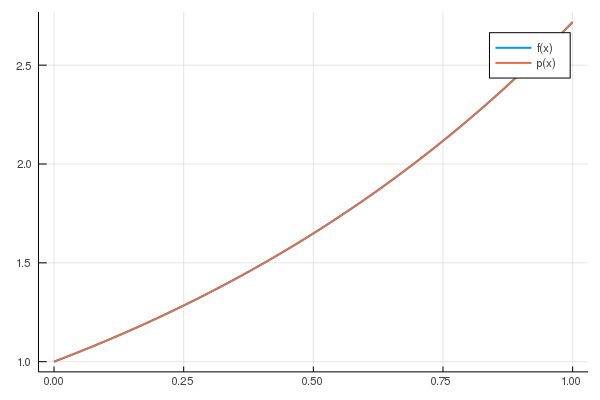
\includegraphics[width=0.5\textwidth]{plots/task5plotf1_5.png}} \hfill
	\subfloat[2.][$n=10$]{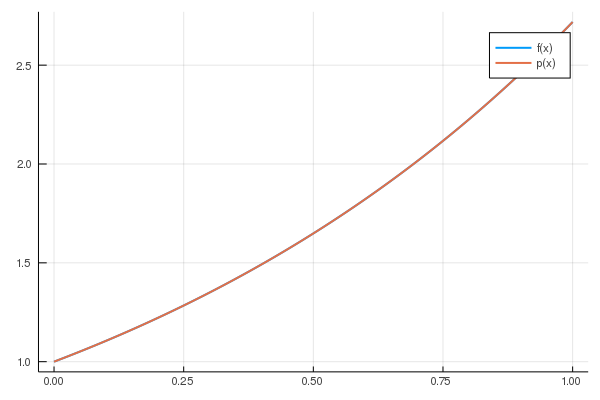
\includegraphics[width=0.5\textwidth]{plots/task5plotf1_10.png}} \hfill
	\subfloat[3.][$n=15$]{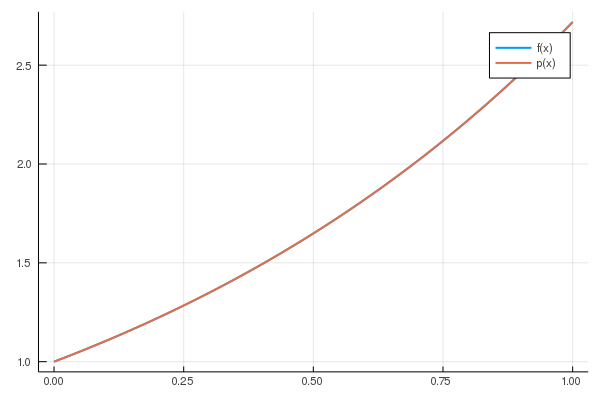
\includegraphics[width=0.5\textwidth]{plots/task5plotf1_15.png}} \hfill
	\caption*{Wykres funkcji $e^{x}$ i jej wielomianu interpolacyjnego dla danego stopnia $n$}
\end{figure}		

\begin{figure}[!htbp]
	\centering
	\subfloat[1.][$n=5$]{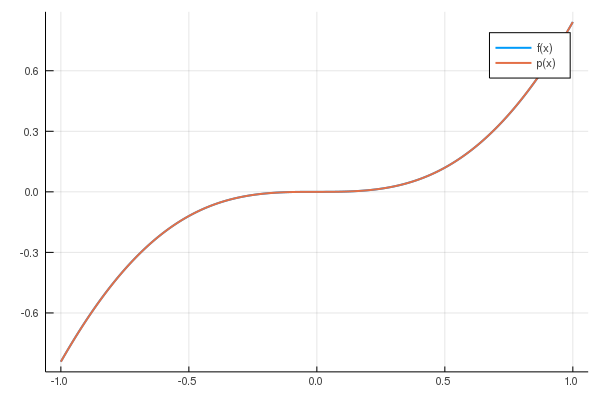
\includegraphics[width=0.5\textwidth]{plots/task5plotf2_5.png}} \hfill
	\subfloat[2.][$n=10$]{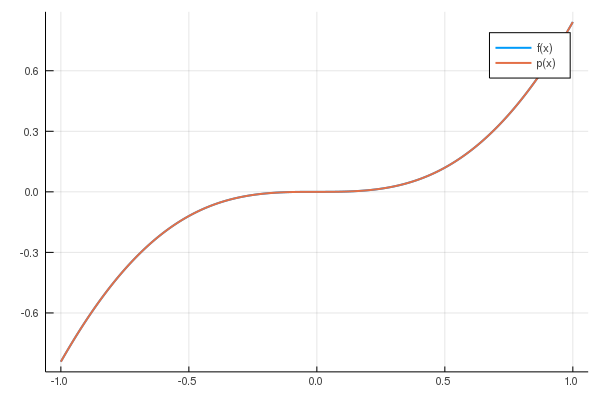
\includegraphics[width=0.5\textwidth]{plots/task5plotf2_10.png}} \hfill
	\subfloat[3.][$n=15$]{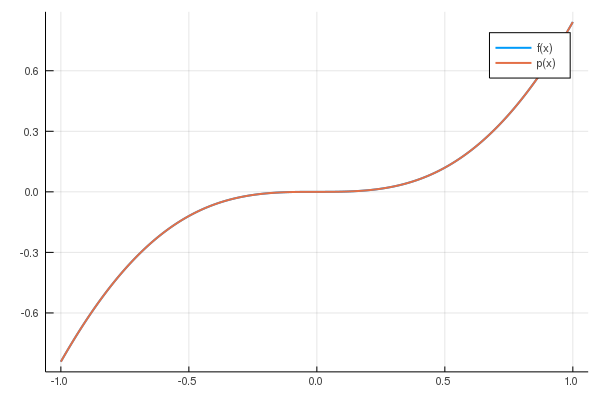
\includegraphics[width=0.5\textwidth]{plots/task5plotf2_15.png}} \hfill
	\caption*{Wykres funkcji $x^2\sin{x}$ i jej wielomianu interpolacyjnego dla danego stopnia $n$}
\end{figure}	





	\clearpage
	
	\section*{Zadanie 6}
	
	Celem zadania było przetestowanie funkcji \texttt{rysujNnfx(f,a,b,n)} (z zadania 4) na następujących przykładach:
	\begin{enumerate}[(a)]
		\item $f(x) = |x|$, $[a, b] = [-1,1]$, $n \in \{5,10,15\}$,
		\item $f(x) = \frac{1}{1+x^2}$, $[a, b] = [-5,5]$, $n \in \{5,10,15\}$.
	\end{enumerate}
Wykresy otrzymane za pomocą metody \texttt{rysujNnfx(f,a,b,n)} prezentują poniższe wykresy.
\begin{figure}[h]
	\centering
	\subfloat[1.][$n=5$]{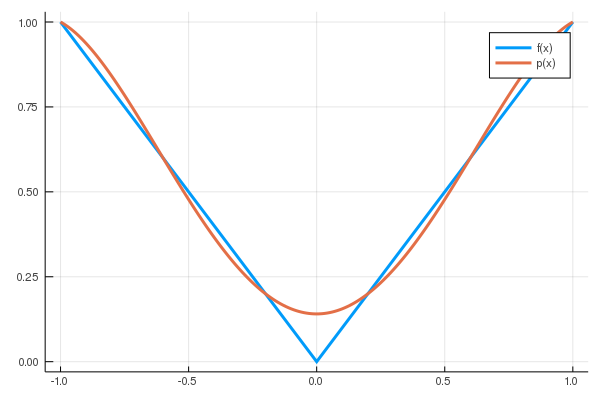
\includegraphics[width=0.5\textwidth]{plots/task6plotf1_5.png}} \hfill
	\subfloat[2.][$n=10$]{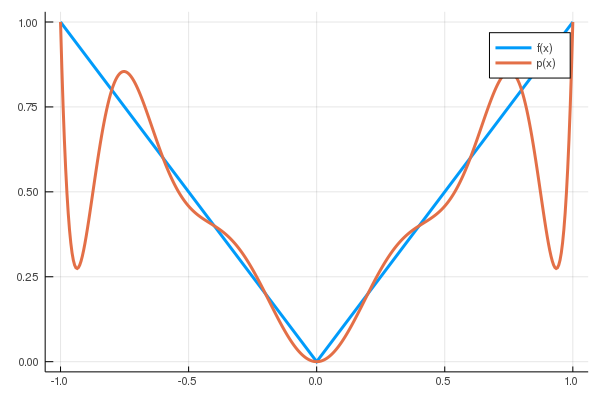
\includegraphics[width=0.5\textwidth]{plots/task6plotf1_10.png}} \hfill
	\subfloat[3.][$n=15$]{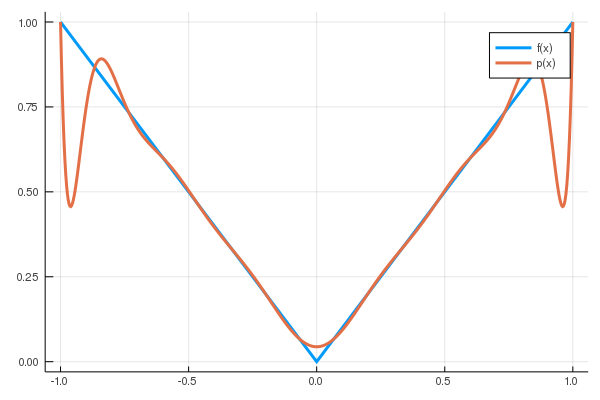
\includegraphics[width=0.5\textwidth]{plots/task6plotf1_15.png}} \hfill
	\subfloat[4.][$n=20$]{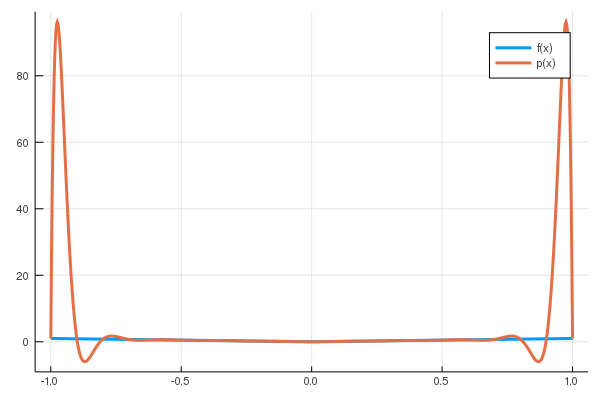
\includegraphics[width=0.5\textwidth]{plots/task6plotf1_20.png}} \hfill
	\caption*{Wykres funkcji $|x|$ i jej wielomianu interpolacyjnego dla danego stopnia $n$}
	\label{fig:3}
\end{figure}		

\begin{figure}[h]
	\centering
	\subfloat[1.][$n=5$]{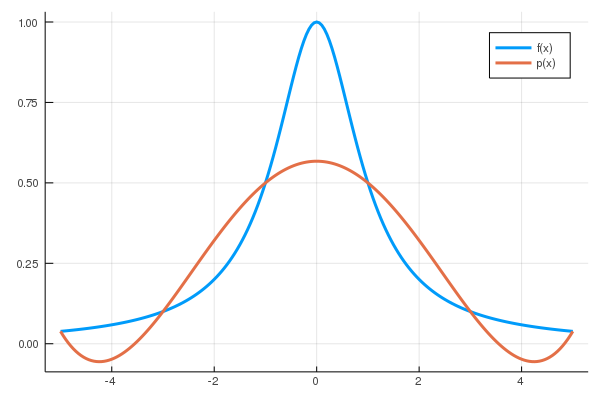
\includegraphics[width=0.5\textwidth]{plots/task6plotf2_5.png}} \hfill
	\subfloat[2.][$n=10$]{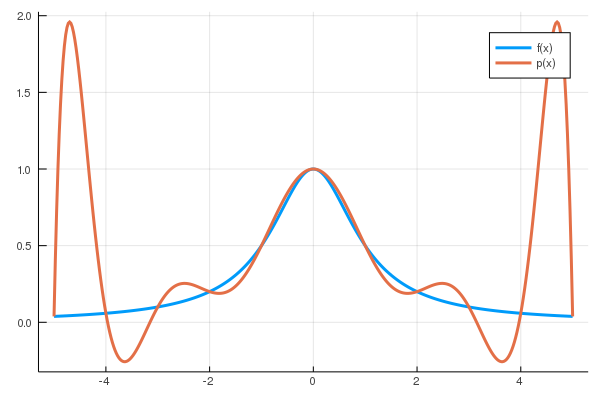
\includegraphics[width=0.5\textwidth]{plots/task6plotf2_10.png}} \hfill
	\subfloat[3.][$n=15$]{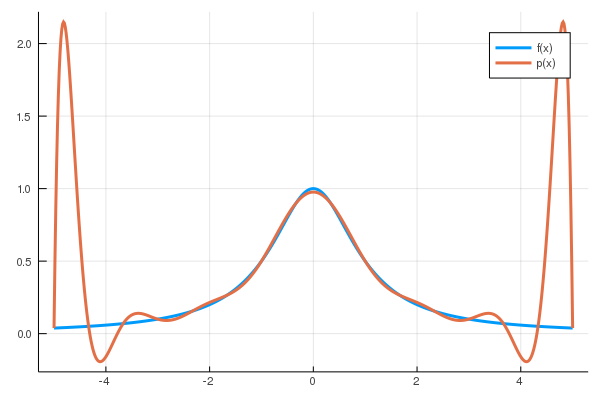
\includegraphics[width=0.5\textwidth]{plots/task6plotf2_15.png}} \hfill
	\subfloat[4.][$n=20$]{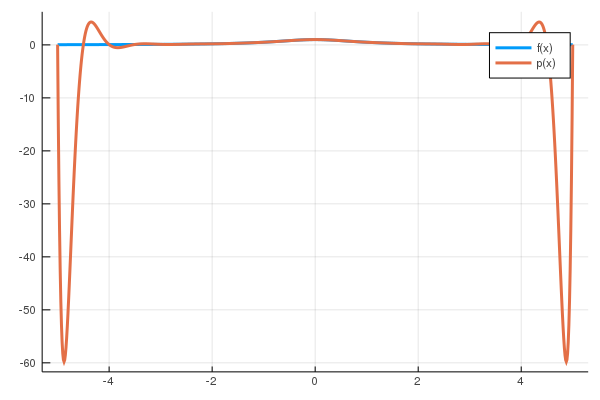
\includegraphics[width=0.5\textwidth]{plots/task6plotf2_20.png}} \hfill
	\caption*{Wykres funkcji $\frac{1}{1+x^2}$ i jej wielomianu interpolacyjnego dla danego stopnia $n$}
	\label{fig:4}
\end{figure}

Widać, że dla funkcji $|x|$ pojawiają się większe odchylenia niż dla funkcji z zadania poprzedniego. Widać też, że wraz ze zwiększaniem stopnia wielomianu odchylenia/błędy, w szczególności na końcach przedziału, znacznie wzrastają. Dla $n=20$ te odchylenia są już na tyle duże, że wykres traci na czytelności. Dla drugiej funkcji sytuacja wygląda tak samo -- wraz ze zwiększaniem stopnia wielomianu błąd rośnie, a błędy najbardziej rosną na końcach przedziału. Jest to sprzeczne z intuicją, ponieważ zwiększajac stopień wielomianu interpolacyjnego oczekujemy lepszego przybliżenia. Zaobserwowane zjawisko nosi nazwę zjawiska Rungego. (Sama funkcja $\frac{1}{1+x^2}$ nazywana jest funkcją Rungego). Polega ono na tym, że dla pewnych funkcji błąd wielomianu
interpolacyjnego wyliczonego za pomocą równoodległych węzłów dąży do nieskończoności wraz ze
wzrostem stopnia tego wielomianu interpolacyjnego.\\
Pojawia się pytanie czy można poprawić dokładność wielomianów interpolacyjnych dla takich funkcji. Z pomocą przychodzą nam węzły Czebyszewa będące pierwiastkami wielomianów Czebyszewa pierwszego rodzaju. Ich użycie zwiększa liczbę węzłów w miejscach, które są trudniejsze do przybliżenia, czyli między innymi na końcach przedziału. Skutkuje to otrzymaniem dokładniejszego przybliżenia. Poniżej znajdują się wykresy z wielomianami interpolacyjnymi stworzonymi na podstawie węzłów Czebyszewa.

\begin{figure}[h]
	\centering
	\subfloat[1.][$n=5$]{\includegraphics[width=0.5\textwidth]{plots/task6ChebyshevPlotf1_5.png}} \hfill
	\subfloat[2.][$n=10$]{\includegraphics[width=0.5\textwidth]{plots/task6ChebyshevPlotf1_10.png}} \hfill
	\subfloat[3.][$n=15$]{\includegraphics[width=0.5\textwidth]{plots/task6ChebyshevPlotf1_15.png}} \hfill
	\subfloat[4.][$n=20$]{\includegraphics[width=0.5\textwidth]{plots/task6ChebyshevPlotf1_20.png}} \hfill
	\caption*{Wykres funkcji $|x|$ i jej wielomianu interpolacyjnego skonstruowanego przy pomocy węzłów Czebyszewa}
	\label{fig:4}
\end{figure}
\begin{figure}[h]
	\centering
	\subfloat[1.][$n=5$]{\includegraphics[width=0.5\textwidth]{plots/task6ChebyshevPlotf2_5.png}} \hfill
	\subfloat[2.][$n=10$]{\includegraphics[width=0.5\textwidth]{plots/task6ChebyshevPlotf2_10.png}} \hfill
	\subfloat[3.][$n=15$]{\includegraphics[width=0.5\textwidth]{plots/task6ChebyshevPlotf2_15.png}} \hfill
	\subfloat[4.][$n=20$]{\includegraphics[width=0.5\textwidth]{plots/task6ChebyshevPlotf2_20.png}} \hfill
	\caption*{Wykres funkcji $\frac{1}{1+x^2}$ i jej wielomianu interpolacyjnego stworzonego przy pomocy węzłów Czebyszewa}
	\label{fig:4}
\end{figure}



\end{document}